\documentclass{beamer}
\usepackage{tcolorbox}
\usepackage{amsmath}
\usepackage{tikz}
\usepackage{pgfplots}
\usepackage{adjustbox}
\usepackage{pgfplots}

%\beamerdefaultoverlayspecification{<+->}
\newcommand{\data}{\mathcal{D}}

\DeclareMathOperator*{\argmin}{arg\,min}

\newcommand\Item[1][]{%
	\ifx\relax#1\relax  \item \else \item[#1] \fi
	\abovedisplayskip=0pt\abovedisplayshortskip=0pt~\vspace*{-\baselineskip}}


\usetheme{metropolis}           % Use metropolis theme


\title{Gradient Descent}
\date{\today}
\author{Nipun Batra}
\institute{IIT Gandhinagar}
\begin{document}
	\maketitle
	
	
	\begin{frame}{Contour Plot And Gradients}
	
	$z = f(x,y) = x^{2} + y^{2}$\\
	
	\begin{columns}
	 \begin{column}{0.6\textwidth}
			\begin{adjustbox}{max totalsize={0.6\textwidth},center}
				
				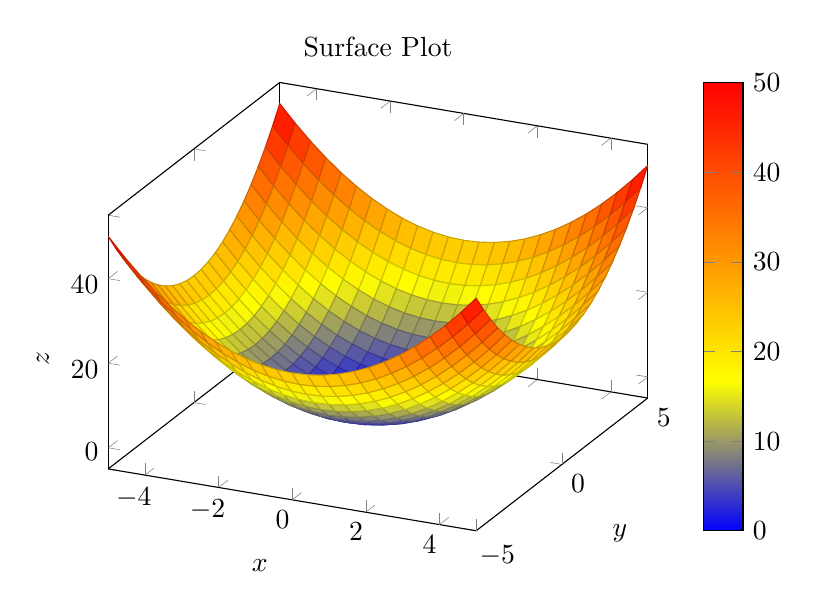
\begin{tikzpicture}
				\begin{axis}[colorbar,xlabel=$x$, ylabel=$y$, zlabel=$z$,title={Surface Plot}]
				\addplot3[
				surf,
				]
				{x^2+y^2};
				\end{axis}
				\end{tikzpicture}
			\end{adjustbox}
			
		\end{column}
	\begin{column}{0.5\textwidth}
			\begin{adjustbox}{max totalsize={0.6\textwidth},center}
				\begin{tikzpicture}
				\begin{axis}
				[
				title={Contour plot, view from top},
				view={0}{90},
				xlabel=$x$,
				ylabel=$y$,
				axis x line*=bottom,
				axis y line*=left,
				xtick align=outside,
				ytick align=outside,
				unit vector ratio*=1 1 1,
				]
				\addplot3[
				contour gnuplot={number=20,}
				]
				{x^2+y^2};
				\addplot3[black,
				quiver={
					u={2*x},
					v={2*y},
					scale arrows=0.1,
				},
				-stealth,samples=10]
				{x^2+y^2};
				\end{axis}
				\end{tikzpicture}
			\end{adjustbox}
		\end{column}
	\end{columns}
	

	
	


\pause Gradient denotes the direction of steepest ascent or the direction in which there is a maximum increase in f(x,y)



\end{frame}

\begin{frame}{Gradient Descent}
\begin{columns}
	
	
	\begin{column}{0.6\textwidth}
		\begin{adjustbox}{max totalsize={\textwidth},center}
			\begin{tikzpicture}
			
			\begin{axis}[
			xlabel=$x$,
			ylabel=$y$,
			xmin=-4.2,
			xmax=4.2,
			ymin=0,
			axis x line*=bottom,
			axis y line*=left,
			xtick align=outside,
			ytick align=outside,
			legend pos=outer north east
			]
			\addplot[mark=none, gray] {x^2};\addlegendentry{$y=x^2$}
			\addplot[mark=none, red] {8.2*x-16.82};\addlegendentry{$y=8.2x-16.82$}
			\addplot[only marks, mark=*]
			coordinates{ % plot 1 data set
				(4.1,16.81)
			}; 
			
			
			
			\end{axis}
			
			\end{tikzpicture}
		\end{adjustbox}
	\end{column}
	
\end{columns}
\begin{itemize}[<+->]
	\item $y = x^2$
	\item Key idea: Go to $x_{1}$ from $x_{0} $ such that $y_{1}< y_{0}$
	\item $\frac{\partial{y}}{\partial{x}} = 2x$
	\item At x = 4.1, we have max. decrease along the direction of -$\frac{\partial{y}}{\partial{x}}$
	\item Equation of tangent at x=4.1: y = 8.2x-16.82
\end{itemize}



\end{frame}

	
		\begin{frame}{Gradient Descent}
	General Optimization Technique\\
	Question: Find minimum y
\end{frame}

\begin{frame}{Gradient Descent}
General Optimization Technique\\
Question: Find minimum y
\begin{itemize}[<+->]
\item Start with some $x_{0}$
\item Till convergence or iterations exhahusted
\begin{itemize}
	\item $x_{i} = x_{i-1} - \alpha\frac{\partial y }{\partial x} x_{i-1}$
\end{itemize}

\end{itemize}
\pause Here, $\alpha$ is the learning rate or step parameter
\end{frame}
	
	\begin{frame}{Iteration 0}
	\begin{columns}
		

		\begin{column}{0.6\textwidth}
			\begin{adjustbox}{max totalsize={\textwidth},center}
				\begin{tikzpicture}
				
					\begin{axis}[
						xlabel=$x$,
						ylabel=$y$,
						xmin=-4.2,
						xmax=4.2,
						axis x line*=bottom,
						axis y line*=left,
						xtick align=outside,
						ytick align=outside,
						legend pos=outer north east
						]
						\addplot[mark=none, gray] {x^2};\addlegendentry{$y=x^2$}
						\addplot[only marks, mark=*]
						coordinates{ % plot 1 data set
							(4.1,16.81)
							}; 
						
					
						
						\end{axis}
				
				\end{tikzpicture}
			\end{adjustbox}
		\end{column}
\begin{column}{0.5\textwidth}
	\begin{adjustbox}{max totalsize={\textwidth},center}
		\begin{tikzpicture}
		\begin{axis}
		[
		title={Contour plot, view from top},
		view={0}{90},
		xlabel=$x$,
		ylabel=$y$,
		axis x line*=bottom,
		axis y line*=left,
		xtick align=outside,
		ytick align=outside,
		unit vector ratio*=1 1 1,
		]
		\addplot3[
		contour gnuplot={number=14,}
		]
		{x^2};
		\addplot[only marks, mark=*]
		coordinates{ % plot 1 data set
			(4.1,0)
		}; 
		\end{axis}
		\end{tikzpicture}
		\end{adjustbox}
	\end{column}
\end{columns}

		\pause Let us start with initial x value of $x_0=4.1$

	
\end{frame}
	
	\begin{frame}{Iteration 1}
	\begin{columns}
		
		
		\begin{column}{0.6\textwidth}
			\begin{adjustbox}{max totalsize={\textwidth},center}
				\begin{tikzpicture}
				
				\begin{axis}[
				xlabel=$x$,
				ylabel=$y$,
				xmin=-4.2,
				xmax=4.2,
				axis x line*=bottom,
				axis y line*=left,
				xtick align=outside,
				ytick align=outside,
				legend pos=outer north east
				]
				\addplot[mark=none, gray] {x^2};\addlegendentry{$y=x^2$}
				\addplot[only marks, mark=*]
				coordinates{ % plot 1 data set
					( 2.46 , 6.05 )
				}; 
				
				
				
				\end{axis}
				
				\end{tikzpicture}
			\end{adjustbox}
		\end{column}
		\begin{column}{0.5\textwidth}
			\begin{adjustbox}{max totalsize={\textwidth},center}
				\begin{tikzpicture}
				\begin{axis}
				[
				title={Contour plot, view from top},
				view={0}{90},
				xlabel=$x$,
				ylabel=$y$,
				axis x line*=bottom,
				axis y line*=left,
				xtick align=outside,
				ytick align=outside,
				unit vector ratio*=1 1 1,
				]
				\addplot3[
				contour gnuplot={number=14,}
				]
				{x^2};
				\addplot[only marks, mark=*]
				coordinates{ % plot 1 data set
					( 2.46 , 0 )
				}; 
				\end{axis}
				\end{tikzpicture}
			\end{adjustbox}
		\end{column}

	\end{columns}
		$x = 4.1 - 0.2\times2\times4.1$
	
\end{frame}
	
	
	
\begin{frame}{Iteration 2 }
\begin{columns}
	
	
	\begin{column}{0.6\textwidth}
		\begin{adjustbox}{max totalsize={\textwidth},center}
			\begin{tikzpicture}
			
			\begin{axis}[
			xlabel=$x$,
			ylabel=$y$,
			xmin=-4.2,
			xmax=4.2,
			axis x line*=bottom,
			axis y line*=left,
			xtick align=outside,
			ytick align=outside,
			legend pos=outer north east
			]
			\addplot[mark=none, gray] {x^2};\addlegendentry{$y=x^2$}
			\addplot[only marks, mark=*]
			coordinates{ % plot 1 data set
				( 1.48 , 2.18 )
			}; 
			
			
			
			\end{axis}
			
			\end{tikzpicture}
		\end{adjustbox}
	\end{column}
	\begin{column}{0.5\textwidth}
		\begin{adjustbox}{max totalsize={\textwidth},center}
			\begin{tikzpicture}
			\begin{axis}
			[
			title={Contour plot, view from top},
			view={0}{90},
			xlabel=$x$,
			ylabel=$y$,
			axis x line*=bottom,
			axis y line*=left,
			xtick align=outside,
			ytick align=outside,
			unit vector ratio*=1 1 1,
			]
			\addplot3[
			contour gnuplot={number=14,}
			]
			{x^2};
			\addplot[only marks, mark=*]
			coordinates{ % plot 1 data set
				( 1.48 , 0 )
			}; 
			\end{axis}
			\end{tikzpicture}
		\end{adjustbox}
	\end{column}
	
\end{columns}
$x = 2.46 - 0.2\times2\times2.46$

\end{frame}


\begin{frame}{Iteration 3}
\begin{columns}
	
	
	\begin{column}{0.6\textwidth}
		\begin{adjustbox}{max totalsize={\textwidth},center}
			\begin{tikzpicture}
			
			\begin{axis}[
			xlabel=$x$,
			ylabel=$y$,
			xmin=-4.2,
			xmax=4.2,
			axis x line*=bottom,
			axis y line*=left,
			xtick align=outside,
			ytick align=outside,
			legend pos=outer north east
			]
			\addplot[mark=none, gray] {x^2};\addlegendentry{$y=x^2$}
			\addplot[only marks, mark=*]
			coordinates{ % plot 1 data set
				( 0.89 , 0.78 )
			}; 
			
			
			
			\end{axis}
			
			\end{tikzpicture}
		\end{adjustbox}
	\end{column}
	\begin{column}{0.5\textwidth}
		\begin{adjustbox}{max totalsize={\textwidth},center}
			\begin{tikzpicture}
			\begin{axis}
			[
			title={Contour plot, view from top},
			view={0}{90},
			xlabel=$x$,
			ylabel=$y$,
			axis x line*=bottom,
			axis y line*=left,
			xtick align=outside,
			ytick align=outside,
			unit vector ratio*=1 1 1,
			]
			\addplot3[
			contour gnuplot={number=14,}
			]
			{x^2};
			\addplot[only marks, mark=*]
			coordinates{ % plot 1 data set
				( 0.89 , 0 )
			}; 
			\end{axis}
			\end{tikzpicture}
		\end{adjustbox}
	\end{column}
	
\end{columns}
$x = 1.48 - 0.2\times2\times1.48$

\end{frame}

\begin{frame}{Iteration 10}
\begin{columns}
	
	
	\begin{column}{0.6\textwidth}
		\begin{adjustbox}{max totalsize={\textwidth},center}
			\begin{tikzpicture}
			
			\begin{axis}[
			xlabel=$x$,
			ylabel=$y$,
			xmin=-4.2,
			xmax=4.2,
			axis x line*=bottom,
			axis y line*=left,
			xtick align=outside,
			ytick align=outside,
			legend pos=outer north east
			]
			\addplot[mark=none, gray] {x^2};\addlegendentry{$y=x^2$}
			\addplot[only marks, mark=*]
			coordinates{ % plot 1 data set
				( 0.02, 0 )
			}; 
			
			
			
			\end{axis}
			
			\end{tikzpicture}
		\end{adjustbox}
	\end{column}
	\begin{column}{0.5\textwidth}
		\begin{adjustbox}{max totalsize={\textwidth},center}
			\begin{tikzpicture}
			\begin{axis}
			[
			title={Contour plot, view from top},
			view={0}{90},
			xlabel=$x$,
			ylabel=$y$,
			axis x line*=bottom,
			axis y line*=left,
			xtick align=outside,
			ytick align=outside,
			unit vector ratio*=1 1 1,
			]
			\addplot3[
			contour gnuplot={number=14,}
			]
			{x^2};
			\addplot[only marks, mark=*]
			coordinates{ % plot 1 data set
				( 0.02 , 0 )
			}; 
			\end{axis}
			\end{tikzpicture}
		\end{adjustbox}
	\end{column}
	
\end{columns}


\end{frame}

	
\begin{frame}{What if $\alpha$ is large?}
The model starts overshooting!
\end{frame}

\begin{frame}{Overshooting}
\begin{center}
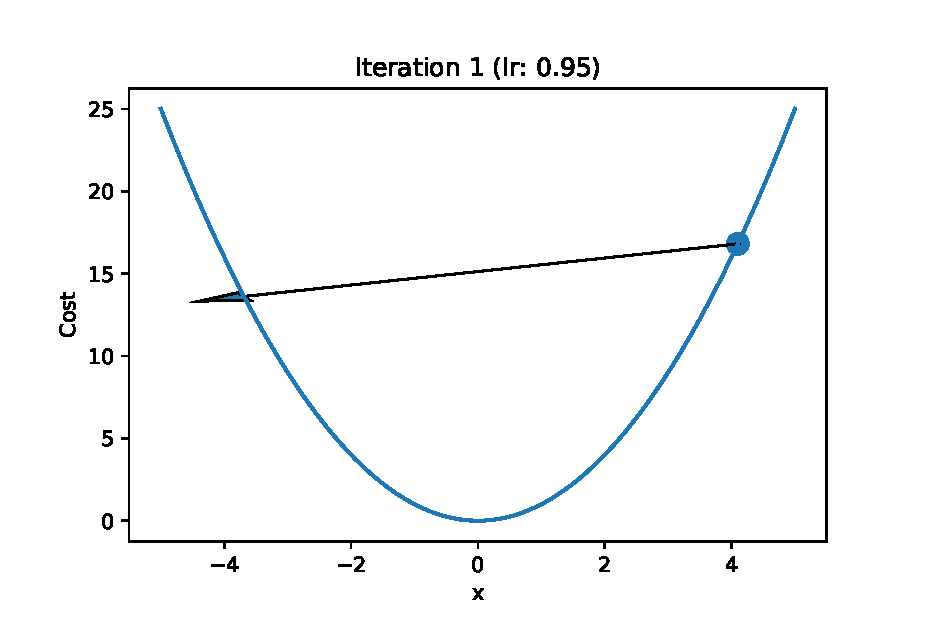
\includegraphics[totalheight=6cm]{gradient-descent/overshooting-1.eps}
\end{center}
\end{frame}

\begin{frame}{Overshooting}
\begin{center}
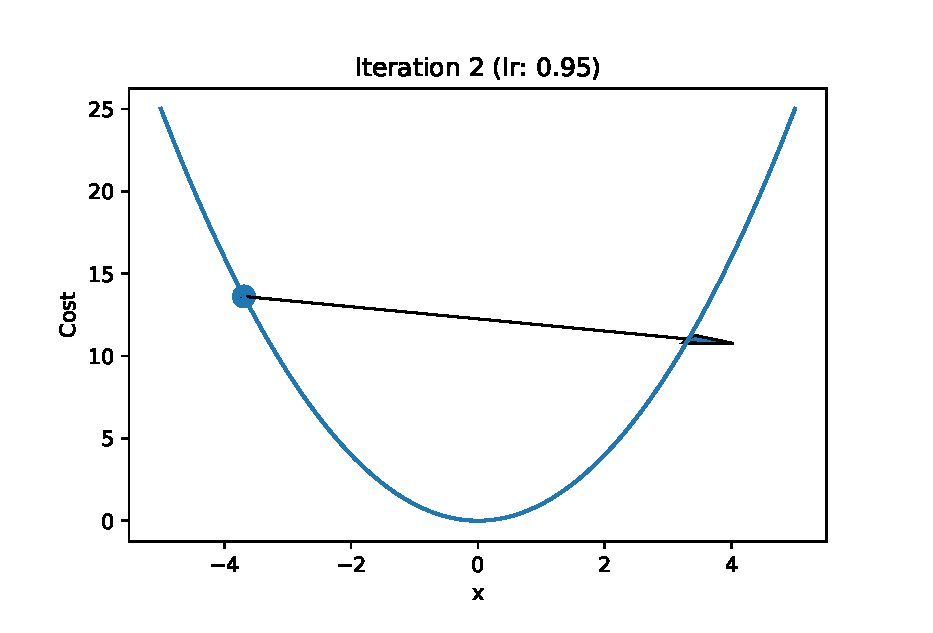
\includegraphics[totalheight=6cm]{gradient-descent/overshooting-2.eps}
\end{center}
\end{frame}

\begin{frame}{Overshooting}
\begin{center}
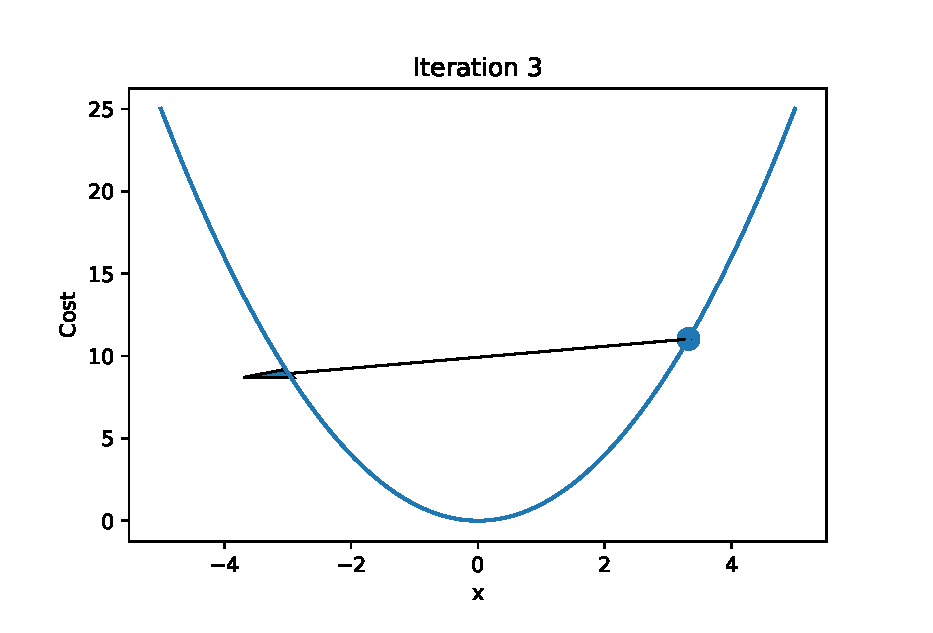
\includegraphics[totalheight=6cm]{gradient-descent/overshooting-3.eps}
\end{center}
\end{frame}

\begin{frame}{Overshooting}
\begin{center}
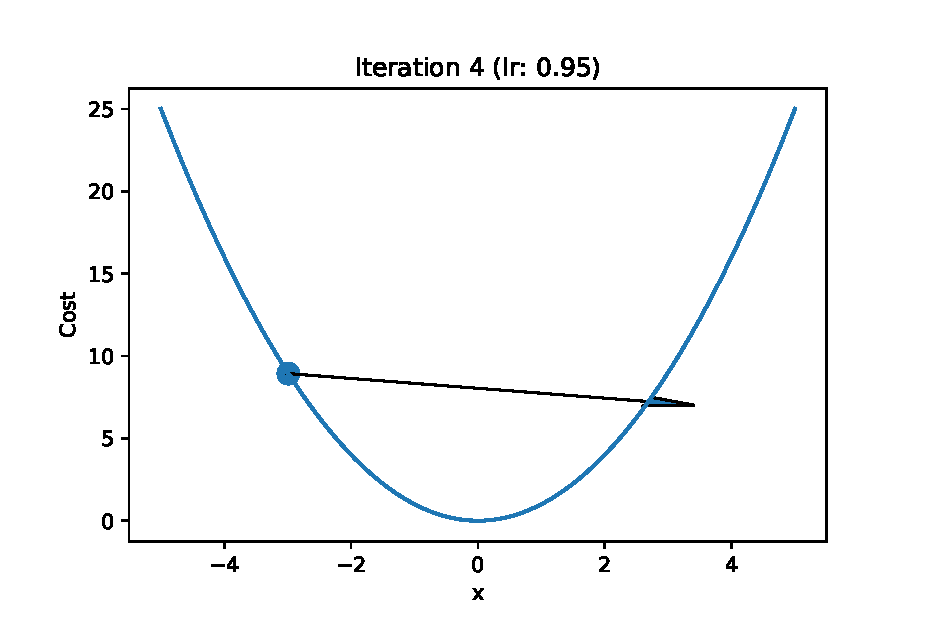
\includegraphics[totalheight=6cm]{gradient-descent/overshooting-4.eps}
\end{center}
\end{frame}

\begin{frame}{Overshooting}
\begin{center}
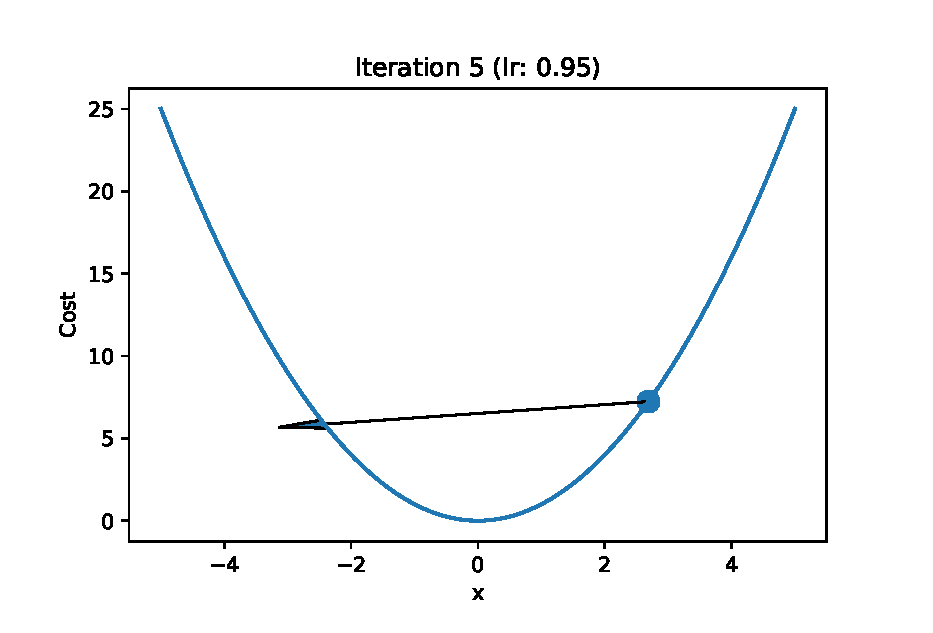
\includegraphics[totalheight=6cm]{gradient-descent/overshooting-5.eps}
\end{center}
\end{frame}

\begin{frame}{Overshooting}
\begin{center}
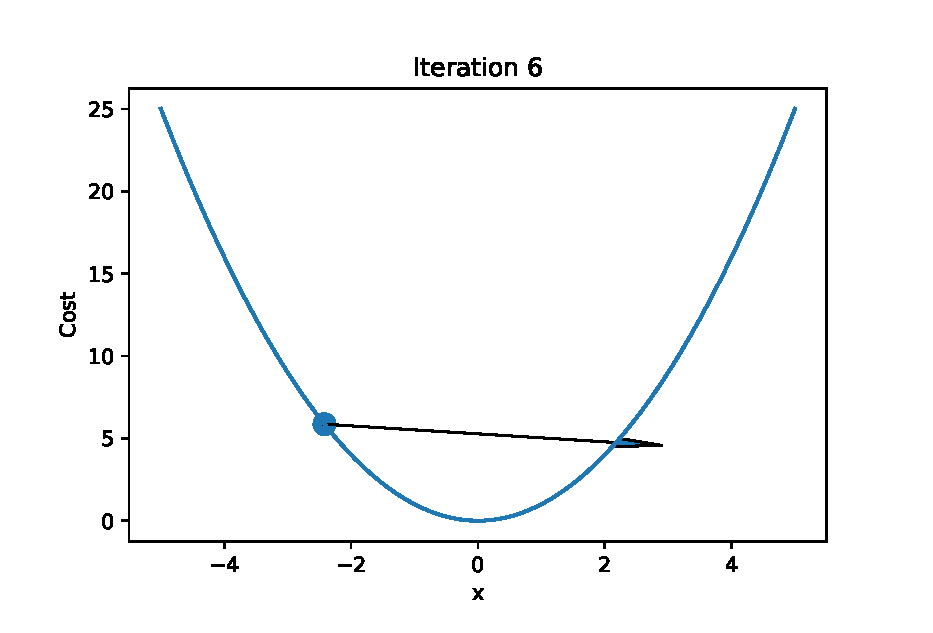
\includegraphics[totalheight=6cm]{gradient-descent/overshooting-6.eps}
\end{center}
\end{frame}

\begin{frame}{Overshooting}
\begin{center}
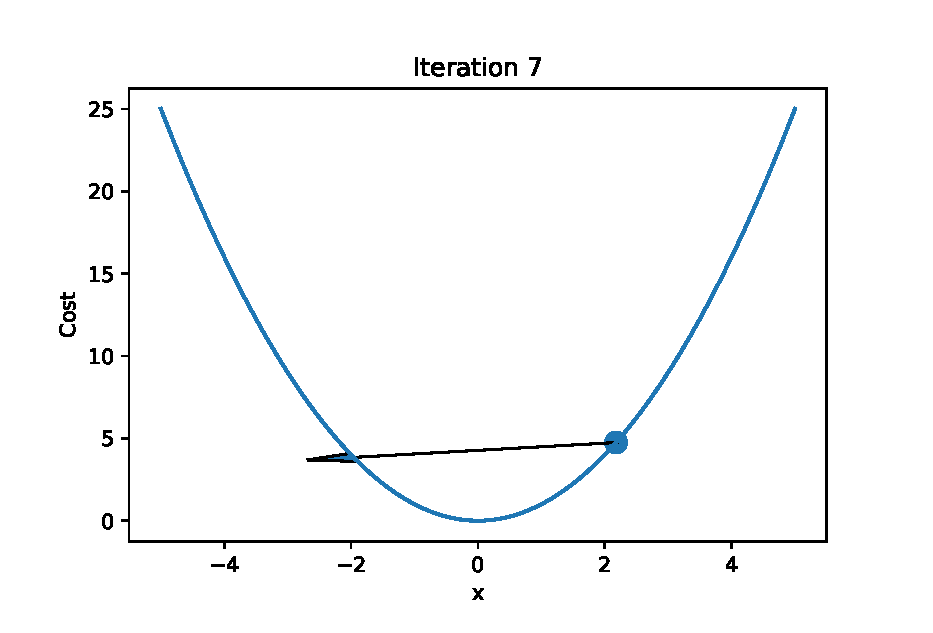
\includegraphics[totalheight=6cm]{gradient-descent/overshooting-7.eps}
\end{center}
\end{frame}

\begin{frame}{Overshooting}
\begin{center}
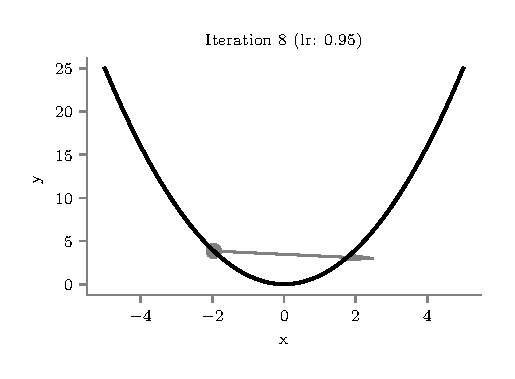
\includegraphics[totalheight=6cm]{gradient-descent/overshooting-8.eps}
\end{center}
\end{frame}

\begin{frame}{Overshooting}
\begin{center}
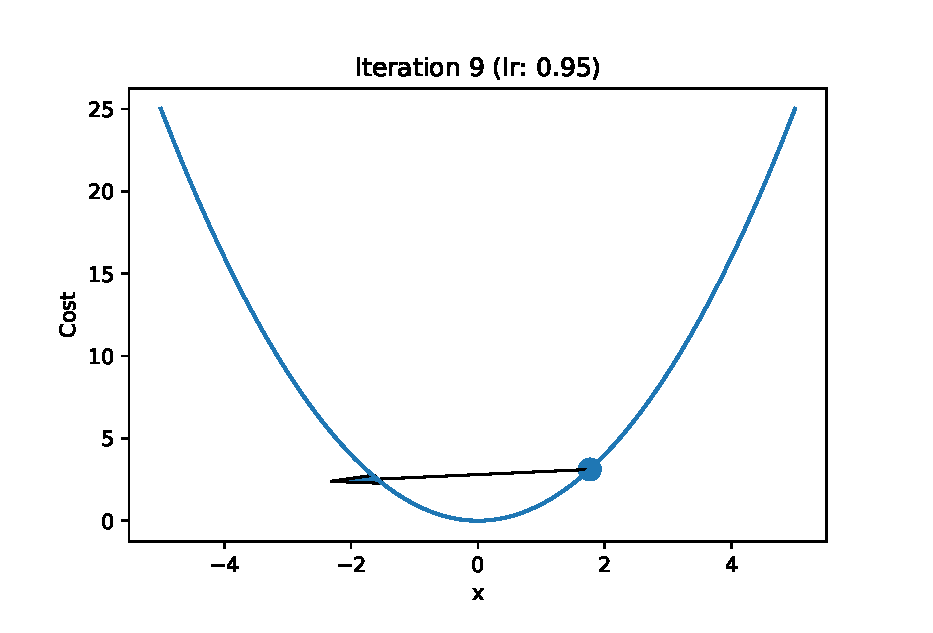
\includegraphics[totalheight=6cm]{gradient-descent/overshooting-9.eps}
\end{center}
\end{frame}

\begin{frame}{Overshooting}
\begin{center}
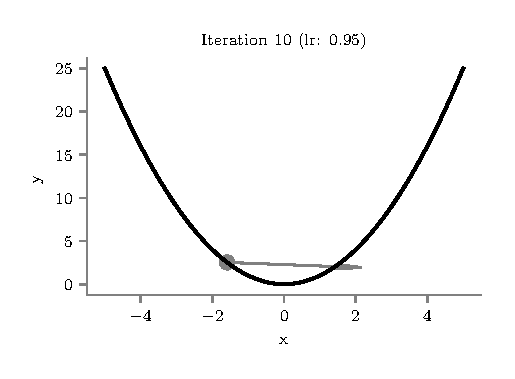
\includegraphics[totalheight=6cm]{gradient-descent/overshooting-10.eps}
\end{center}
\end{frame}

\begin{frame}{What if $\alpha$ is very small?}
Then the rate of convergence is small. It takes more time for a model to reach the minimum cost!
\end{frame}

\begin{frame}{Slow Convergence}
\begin{center}
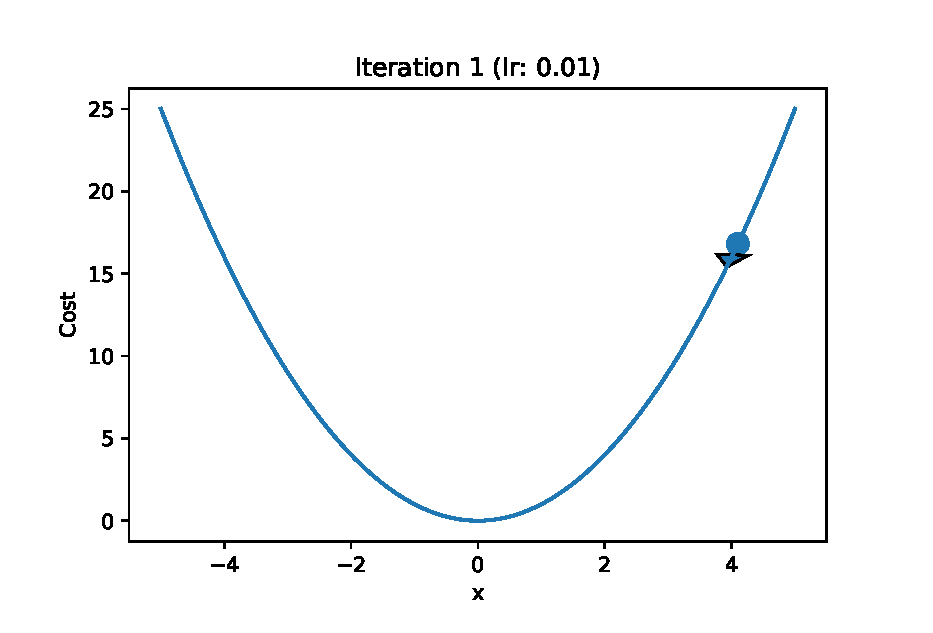
\includegraphics[totalheight=6cm]{gradient-descent/undershooting-1.eps}
\end{center}
\end{frame}

\begin{frame}{Slow Convergence}
\begin{center}
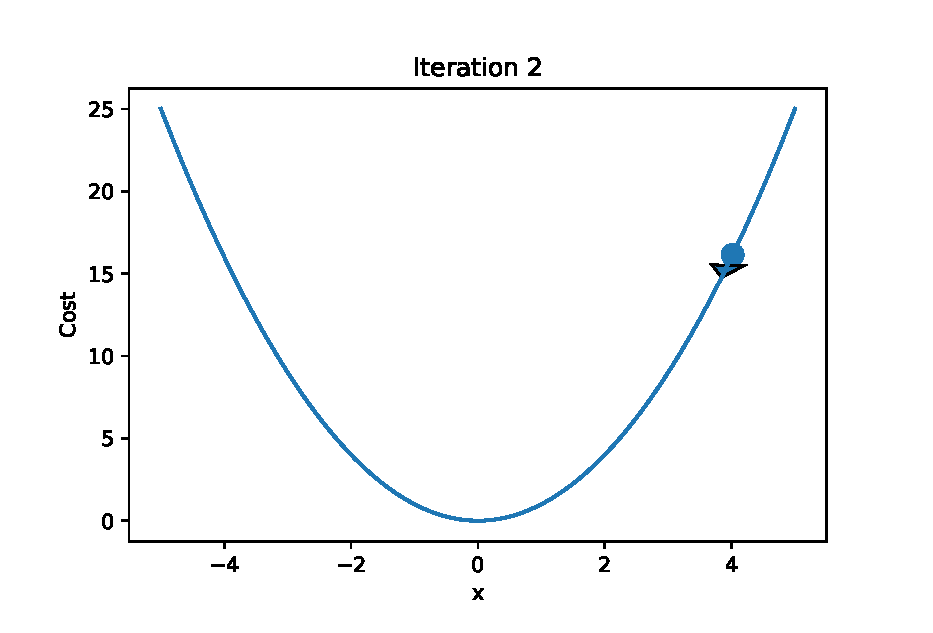
\includegraphics[totalheight=6cm]{gradient-descent/undershooting-2.eps}
\end{center}
\end{frame}

\begin{frame}{Slow Convergence}
\begin{center}
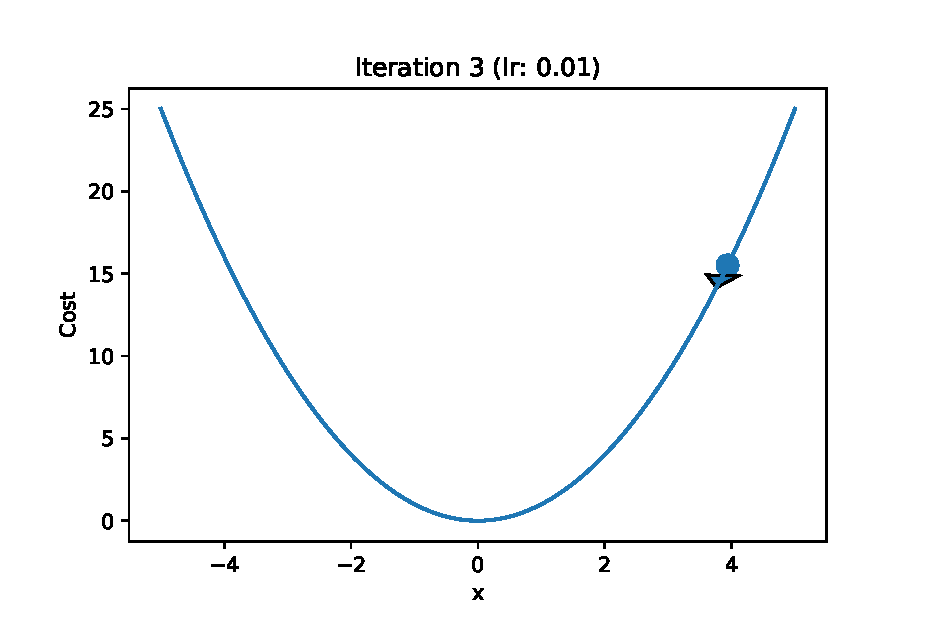
\includegraphics[totalheight=6cm]{gradient-descent/undershooting-3.eps}
\end{center}
\end{frame}

\begin{frame}{Slow Convergence}
\begin{center}
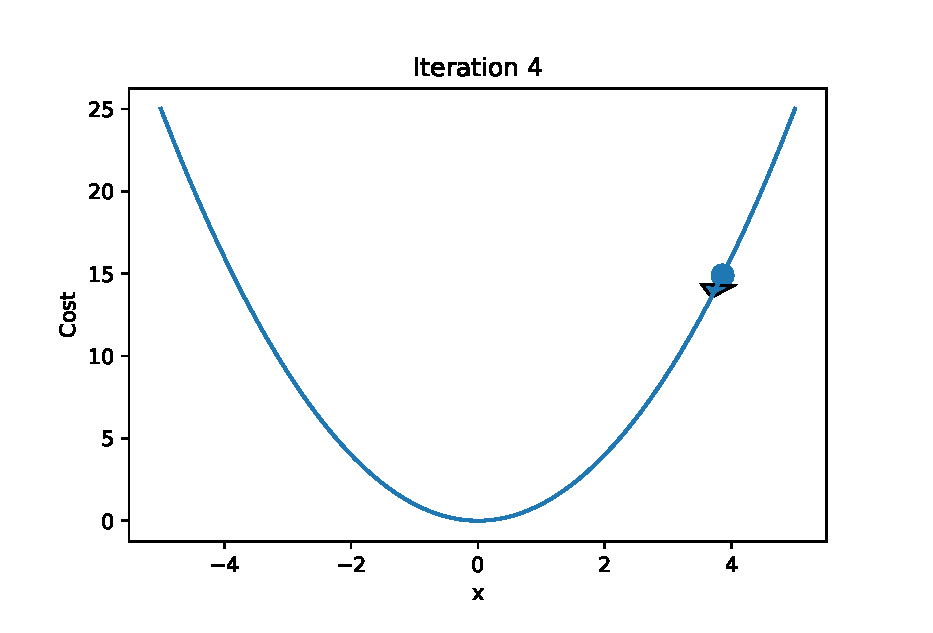
\includegraphics[totalheight=6cm]{gradient-descent/undershooting-4.eps}
\end{center}
\end{frame}

\begin{frame}{Slow Convergence}
\begin{center}
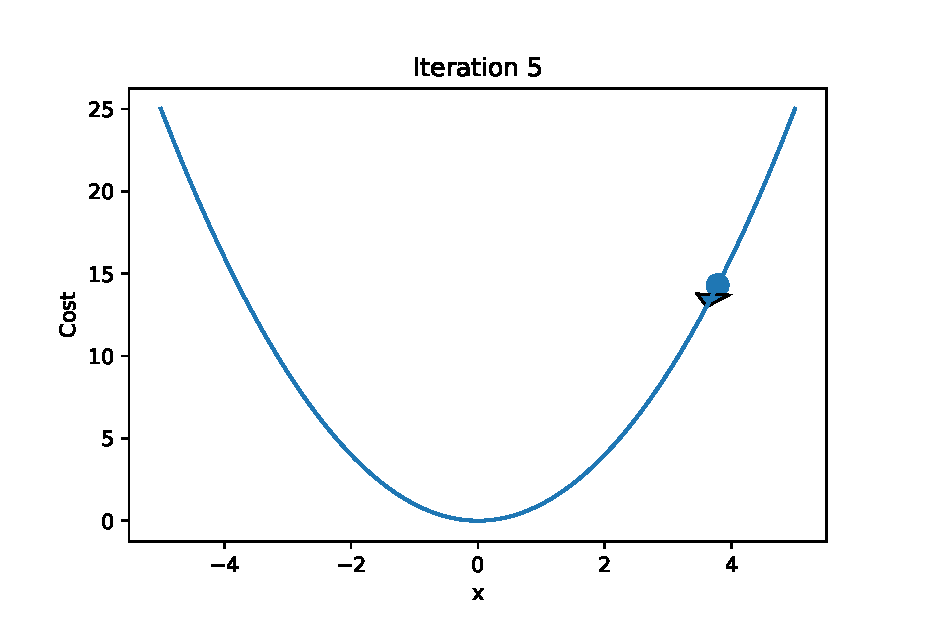
\includegraphics[totalheight=6cm]{gradient-descent/undershooting-5.eps}
\end{center}
\end{frame}

\begin{frame}{Slow Convergence}
\begin{center}
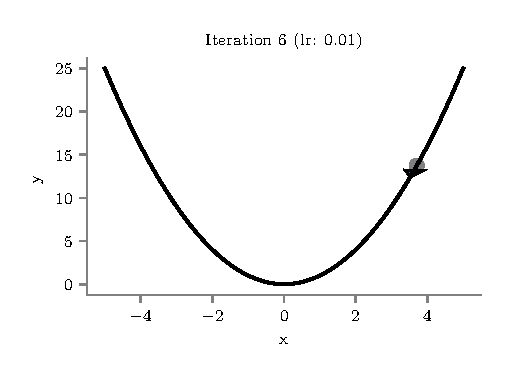
\includegraphics[totalheight=6cm]{gradient-descent/undershooting-6.eps}
\end{center}
\end{frame}

\begin{frame}{Slow Convergence}
\begin{center}
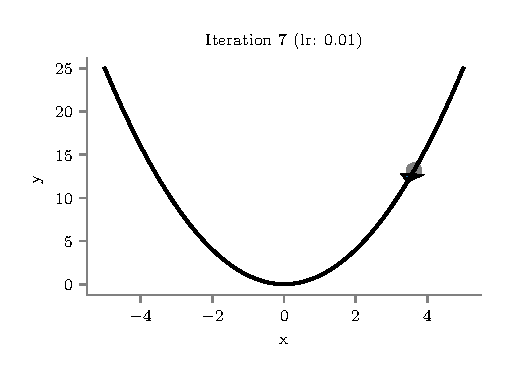
\includegraphics[totalheight=6cm]{gradient-descent/undershooting-7.eps}
\end{center}
\end{frame}

\begin{frame}{Slow Convergence}
\begin{center}
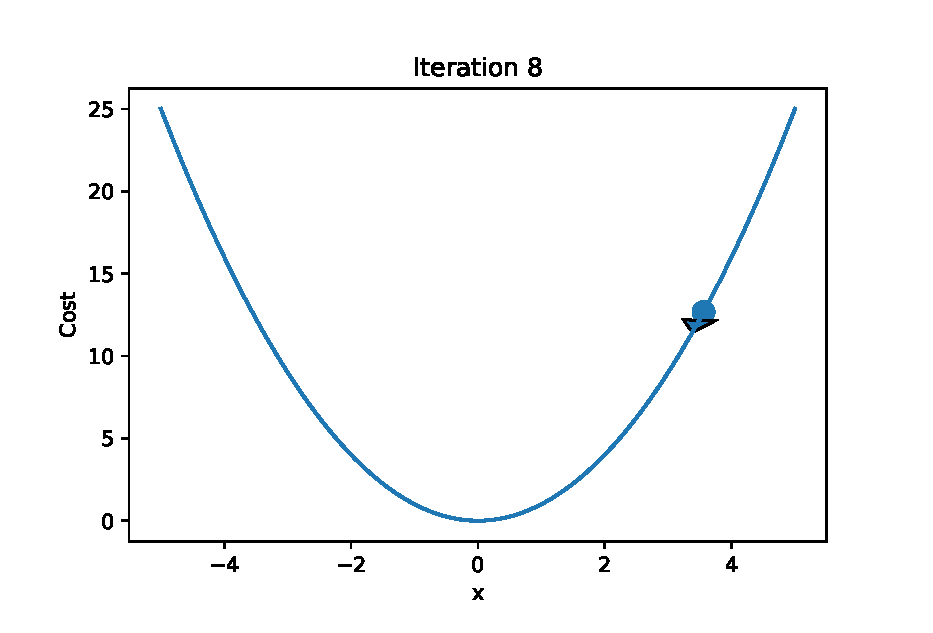
\includegraphics[totalheight=6cm]{gradient-descent/undershooting-8.eps}
\end{center}
\end{frame}

\begin{frame}{Slow Convergence}
\begin{center}
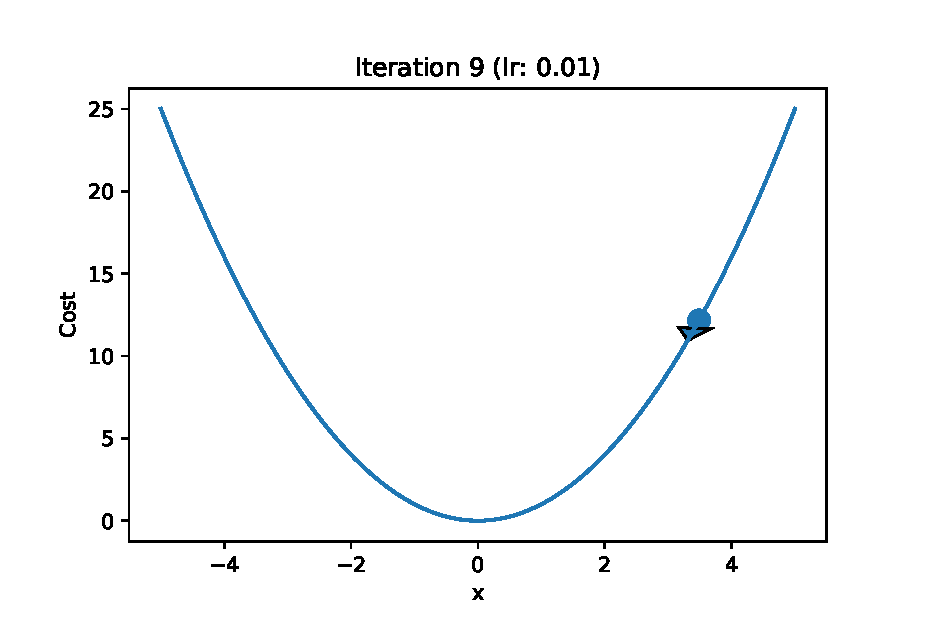
\includegraphics[totalheight=6cm]{gradient-descent/undershooting-9.eps}
\end{center}
\end{frame}

\begin{frame}{Slow Convergence}
\begin{center}
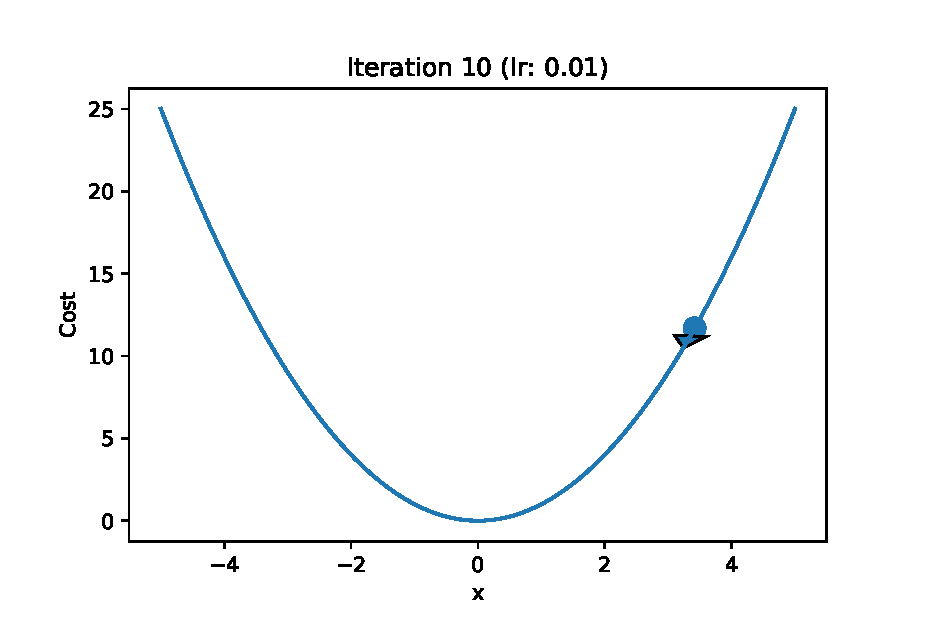
\includegraphics[totalheight=6cm]{gradient-descent/undershooting-10.eps}
\end{center}
\end{frame}

	\begin{frame}{Local Minima}
\begin{center}
	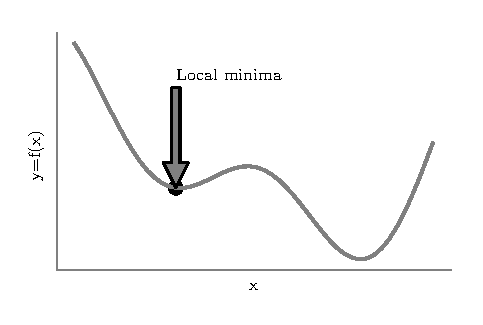
\includegraphics[totalheight=6cm]{gradient-descent/local-minima.eps}
\end{center}
\end{frame}

	\begin{frame}{Gradient Descent for Linear Regression}

\begin{equation*}
\sum \epsilon_{i}^{2} = \sum (y_{i} - (\theta_{0} + \theta_{1}x_{i}))^{2}
\end{equation*}

\end{frame}

\begin{frame}{Gradient Descent Algorithm}

Start with random values of $\theta_{0}$ and $\theta_{1}$\\
Till convergence
\begin{itemize}
\item $\theta_{0} = \theta_{0} - \cfrac{\partial}{\partial \theta_{0}} (\sum \epsilon_{i}^{2}) $
\item $\theta_{1} = \theta_{1} - \cfrac{\partial}{\partial \theta_{1}} (\sum \epsilon_{i}^{2}) $
\end{itemize}

\textbf{The updates have to be done simultaneously!}
\end{frame}

\begin{frame}{Gradient Descent Algorithm}

\begin{itemize}
\item $\cfrac{\partial}{\partial \theta_{0}} (\sum \epsilon_{i}^{2}) = 2\sum (y_{i} - (\theta_{0} + \theta_{1}x{i}))(-1)$
$\cfrac{\partial}{\partial \theta_{1}} (\sum \epsilon_{i}^{2}) = 2\sum (y_{i} - (\theta_{0} + \theta_{1}x{i}))(-x_{i})$
\end{itemize}
\end{frame}

	\begin{frame}{Gradient Descent : Example}
Learn $y = \theta_0 + \theta_1 x$ on following dataset, using gradient descent where initially $(\theta_0, \theta_1) = (4,0)$ and step-size, $\alpha  = 0.1$, for 2 iterations. 
\begin{table}[]
	\centering
	\label{tab:my-table}
	\begin{tabular}{|c|c|}
		\hline
		\textbf{x} & \textbf{y} \\ \hline
		1 & 1 \\ \hline
		2 & 2 \\ \hline
		3 & 3 \\ \hline
	\end{tabular}
\end{table}
\end{frame}



\begin{frame}{Gradient Descent : Example}
Our predictor, $\hat{y} = \theta_0 + \theta_1x$\\
\vspace{1cm}
Error for $i^{th}$ datapoint, $\epsilon_i = y_i - \hat{y_i}$\\
$\epsilon_1 = 1 - \theta_0 - \theta_1$ \\
$\epsilon_2 = 2 - \theta_0 - 2\theta_1$ \\
$\epsilon_3 = 3 - \theta_0 - 3\theta_1$ \\

\vspace{1cm}
MSE = $\dfrac{\epsilon_1^2 + \epsilon_2^2 + \epsilon_3^2}{3}$ = $\dfrac{14 + 3\theta_0^2 + 14\theta_1^2 -12\theta_0 - 28\theta_1 + 12\theta_0\theta_1}{3}$\\
\end{frame}

	\begin{frame}{Difference between SSE and MSE}



\begin{equation*}
\sum \epsilon_{i}^{2} \textit{ increases as the number of examples increase}
\end{equation*}

So, we use MSE

\begin{equation*}
\textit{MSE} = \frac{1}{n} \sum \epsilon_{i}^{2}
\end{equation*}

Here $n$ denotes the number of samples



\end{frame}

\begin{frame}{Iteration 0}

MSE = $\frac{1}{3}(14+3\theta_{0}^{2}+14\theta_{1}^{2}-12\theta_{0}-28\theta_{1}+12\theta_{0}\theta_{1})$\\

\begin{columns}
	\begin{column}{0.6\textwidth}
		\begin{adjustbox}{max totalsize={\textwidth},center}
			
			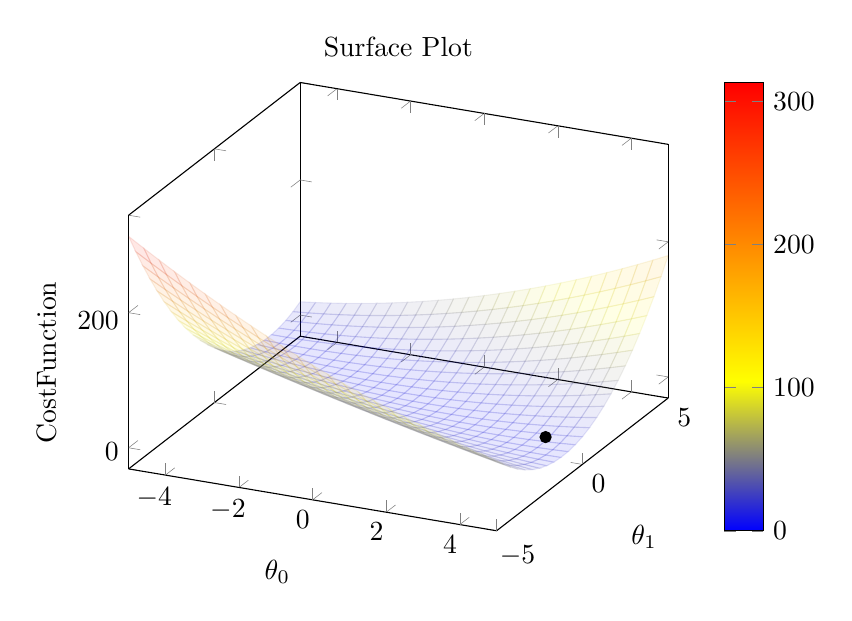
\begin{tikzpicture}
			\begin{axis}[colorbar,xlabel=$\theta_0$, ylabel=$\theta_1$, zlabel=$\mathrm{Cost Function}$,title={Surface Plot}]
			\addplot3[
			surf,opacity=0.1,
			]
			{(14 + 3*x^2 +14*y^2 -12*x - 28*y + 12*x*y)/3};
			\addplot[only marks, mark=*]
			coordinates{ % plot 1 data set
				( 4 , 0 )
			}; 
			\end{axis}
			\end{tikzpicture}
		\end{adjustbox}
		
	\end{column}
 \begin{column}{0.5\textwidth}
		\begin{adjustbox}{max totalsize={\textwidth},center}
			\begin{tikzpicture}
			\begin{axis}
			[
			title={Contour plot, view from top},
			view={0}{90},
			xlabel=$\theta_0$,
			ylabel=$\theta_1$,
			axis x line*=bottom,
			axis y line*=left,
			xtick align=outside,
			ytick align=outside,
			unit vector ratio*=1 1 1,
			]
			\addplot3[
			contour gnuplot={number=25,}
			]
			{(14 + 3*x^2 +14*y^2 -12*x - 28*y + 12*x*y)/3};
			\addplot[only marks, mark=*]
			coordinates{ % plot 1 data set
				( 4 , 0 )
			}; 
			\end{axis}
			\end{tikzpicture}
		\end{adjustbox}
	\end{column}
\end{columns}




\end{frame}



\begin{frame}{Gradient Descent : Example}
$\dfrac{\partial MSE}{\partial \theta_0} = \dfrac{2\sum\limits_i \left( y_i - \theta_0 -\theta_1x_i \right)\left(-1\right)}{N} = \dfrac{2\sum\limits_i \epsilon_i\left(-1\right)}{N}$  

\vspace{2cm}
$\dfrac{\partial MSE}{\partial \theta_1} = \dfrac{2\sum\limits_i \left( y_i - \theta_0 -\theta_1x_i \right)\left(-x_i\right)}{N} = \dfrac{2\sum\limits_i \epsilon_i\left(-x_i\right)}{N}$ 
\end{frame}

\begin{frame}{Gradient Descent : Example}
\textbf{Iteration 1}\\
\vspace{0.5cm}
$\theta_0 = \theta_0 - \alpha\dfrac{\partial MSE}{\partial \theta_0}$\\ 
\vspace{0.5cm}
\only<2->{
$\theta_0 = 4 - 0.2\frac{\left( (1 - (4 + 0))(-1) + (2 - (4 + 0))(-1) +  (3 - (4 + 0))(-1)  \right)}{3}$\\

\vspace{0.5cm}
$\theta_0 = 3.6$
\vspace{0.5cm}
}

$\theta_1 = \theta_1 - \alpha\dfrac{\partial MSE}{\partial \theta_1}$\\ 
\vspace{0.5cm}
\only<3->{
$\theta_1	 = 0 - 0.2\frac{\left( (1 - (4 + 0))(-1) + (2 - (4 + 0))(-2) +  (3 - (4 + 0))(-3)  \right)}{3} $\\
\vspace{0.5cm}
$\theta_1 = -0.67$
}
\end{frame}

\begin{frame}{Iteration 1}

MSE = $\frac{1}{3}(14+3\theta_{0}^{2}+14\theta_{1}^{2}-12\theta_{0}-28\theta_{1}+12\theta_{0}\theta_{1})$\\

\begin{columns}
	\pause \begin{column}{0.6\textwidth}
		\begin{adjustbox}{max totalsize={\textwidth},center}
			
			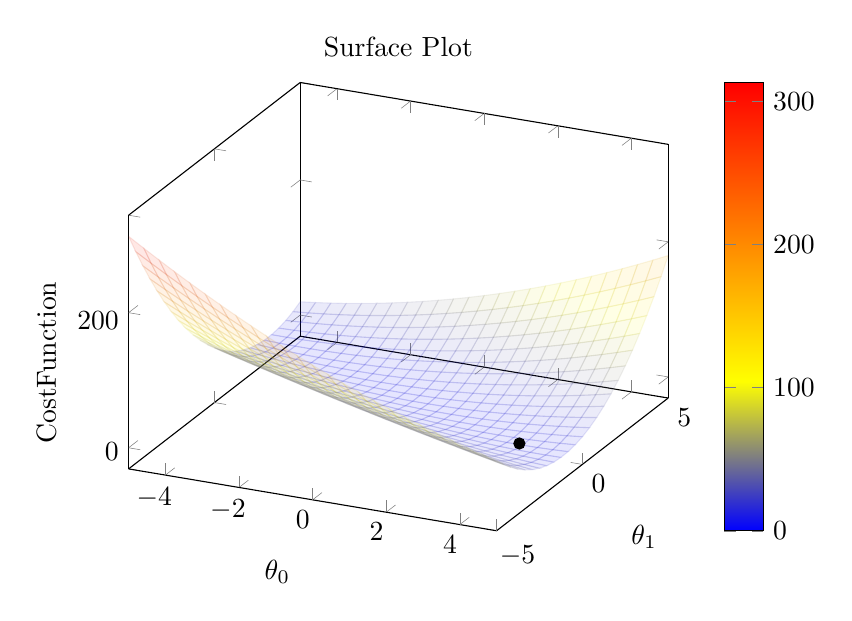
\begin{tikzpicture}
			\begin{axis}[colorbar,xlabel=$\theta_0$, ylabel=$\theta_1$, zlabel=$\mathrm{Cost Function}$,title={Surface Plot}]
			\addplot3[
			surf,opacity=0.1,
			]
			{(14 + 3*x^2 +14*y^2 -12*x - 28*y + 12*x*y)/3};
			\addplot[only marks, mark=*]
			coordinates{ % plot 1 data set
				( 3.6 , -0.67 )
			}; 
			\end{axis}
			\end{tikzpicture}
		\end{adjustbox}
		
	\end{column}
	\pause \begin{column}{0.5\textwidth}
		\begin{adjustbox}{max totalsize={\textwidth},center}
			\begin{tikzpicture}
			\begin{axis}
			[
			title={Contour plot, view from top},
			view={0}{90},
			xlabel=$\theta_0$,
			ylabel=$\theta_1$,
			axis x line*=bottom,
			axis y line*=left,
			xtick align=outside,
			ytick align=outside,
			unit vector ratio*=1 1 1,
			]
			\addplot3[
			contour gnuplot={number=25,}
			]
			{(14 + 3*x^2 +14*y^2 -12*x - 28*y + 12*x*y)/3};
			\addplot[only marks, mark=*]
			coordinates{ % plot 1 data set
				( 3.6 , -0.67 )
			}; 
			\end{axis}
			\end{tikzpicture}
		\end{adjustbox}
	\end{column}
\end{columns}




\end{frame}



\begin{frame}{Gradient Descent : Example}
\textbf{Iteration 2}\\
\vspace{0.5cm}
$\theta_0 = \theta_0 - \alpha\dfrac{\partial MSE}{\partial \theta_0}$\\ 
\vspace{0.5cm}
\only<2->{
$\theta_0 = 3.6 - 0.2\frac{\left( (1 - (3.6  - 0.67))(-1) + (2 - (3.6  - 0.67\times 2))(-1) +  (3 - (3.6  - 0.67\times3))(-1)  \right)}{3}$\\ 
\vspace{0.5cm}
$\theta_0 = 3.54$\\
}

\vspace{0.5cm}

$\theta_1 = \theta_1 - \alpha\dfrac{\partial MSE}{\partial \theta_1}$\\ 
\vspace{0.5cm}
\only<3->{
$\theta_0 = 3.6 - 0.2\frac{\left( (1 - (3.6  - 0.67))(-1) + (2 - (3.6  - 0.67\times 2))(-2) +  (3 - (3.6  - 0.67\times3))(-3)  \right)}{3}$\\ 
\vspace{0.5cm}
$\theta_0 = -0.55$\\
}

\end{frame}



\begin{frame}{Iteration 2}

MSE = $\frac{1}{3}(14+3\theta_{0}^{2}+14\theta_{1}^{2}-12\theta_{0}-28\theta_{1}+12\theta_{0}\theta_{1})$\\

\begin{columns}
	\begin{column}{0.6\textwidth}
		\begin{adjustbox}{max totalsize={\textwidth},center}
			
			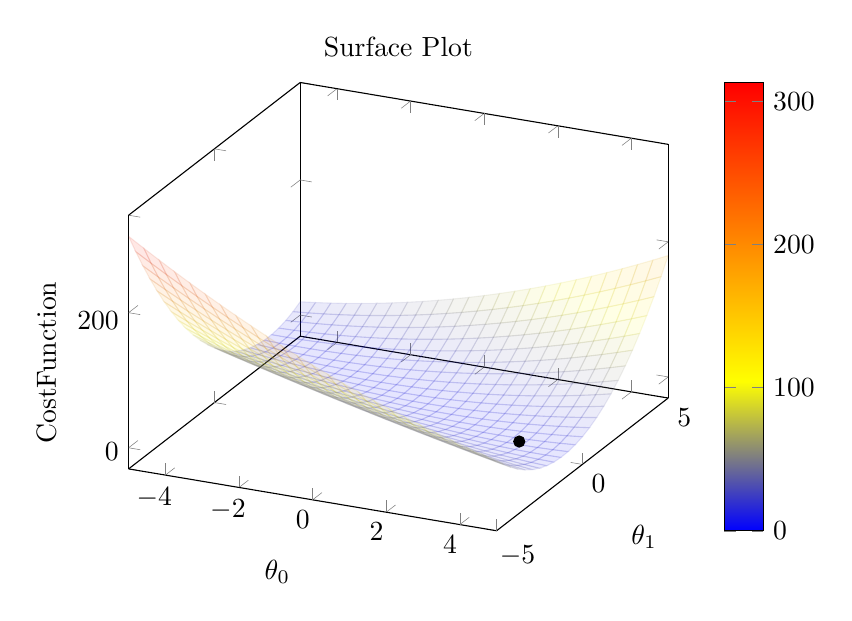
\begin{tikzpicture}
			\begin{axis}[colorbar,xlabel=$\theta_0$, ylabel=$\theta_1$, zlabel=$\mathrm{Cost Function}$,title={Surface Plot}]
			\addplot3[
			surf,opacity=0.1,
			]
			{(14 + 3*x^2 +14*y^2 -12*x - 28*y + 12*x*y)/3};
			\addplot[only marks, mark=*]
			coordinates{ % plot 1 data set
				( 3.54 , -0.55 )
			}; 
			\end{axis}
			\end{tikzpicture}
		\end{adjustbox}
		
	\end{column}
	\begin{column}{0.5\textwidth}
		\begin{adjustbox}{max totalsize={\textwidth},center}
			\begin{tikzpicture}
			\begin{axis}
			[
			title={Contour plot, view from top},
			view={0}{90},
			xlabel=$\theta_0$,
			ylabel=$\theta_1$,
			axis x line*=bottom,
			axis y line*=left,
			xtick align=outside,
			ytick align=outside,
			unit vector ratio*=1 1 1,
			]
			\addplot3[
			contour gnuplot={number=25,}
			]
			{(14 + 3*x^2 +14*y^2 -12*x - 28*y + 12*x*y)/3};
			\addplot[only marks, mark=*]
			coordinates{ % plot 1 data set
				( 3.54 , -0.55 )
			}; 
			\end{axis}
			\end{tikzpicture}
		\end{adjustbox}
	\end{column}
\end{columns}
\end{frame}


\begin{frame}{Cost v/s Iterations ($\alpha=0.1$)}
\begin{figure}
	\centering
	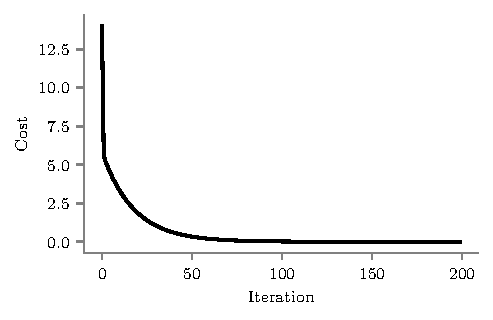
\includegraphics[width=0.7\linewidth]{gradient-descent/gd-iter-cost}
	\label{fig:gd-iter-cost}
\end{figure}

\end{frame}


\begin{frame}{Fit at iteration 0}
\begin{figure}
	\centering
	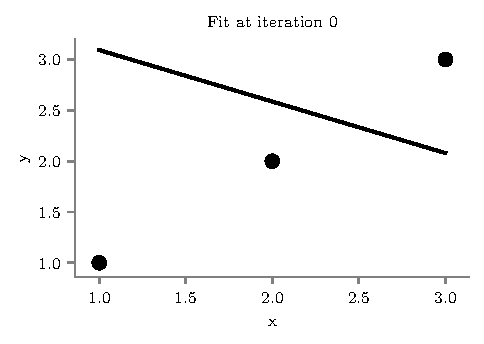
\includegraphics[width=0.7\linewidth]{gradient-descent/fit-iteration-0.pdf}
\end{figure}
\end{frame}

\begin{frame}{Fit at iteration 20}
\begin{figure}
	\centering
	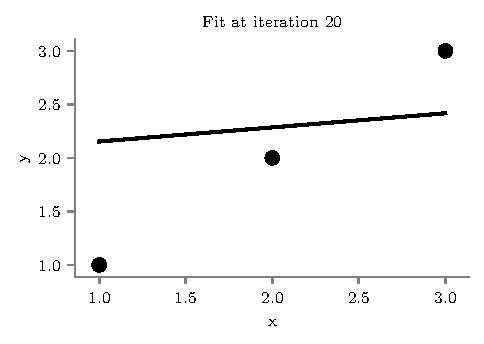
\includegraphics[width=0.7\linewidth]{gradient-descent/fit-iteration-20.pdf}
\end{figure}
\end{frame}

\begin{frame}{Fit at iteration 40}
\begin{figure}
	\centering
	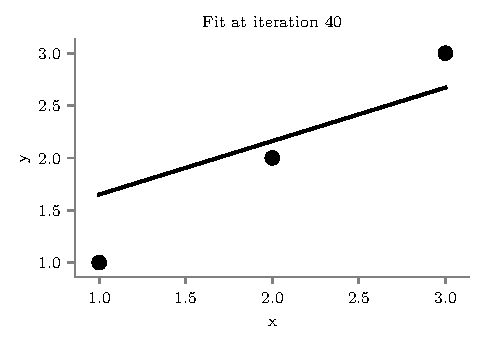
\includegraphics[width=0.7\linewidth]{gradient-descent/fit-iteration-40.pdf}
\end{figure}
\end{frame}

	
\begin{frame}{Fit at iteration 60}
\begin{figure}
	\centering
	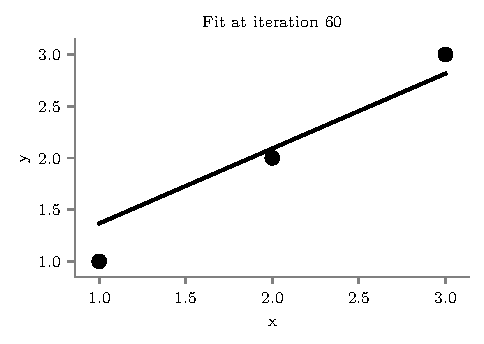
\includegraphics[width=0.7\linewidth]{gradient-descent/fit-iteration-60.pdf}
\end{figure}
\end{frame}

\begin{frame}{Fit at iteration 80}
\begin{figure}
	\centering
	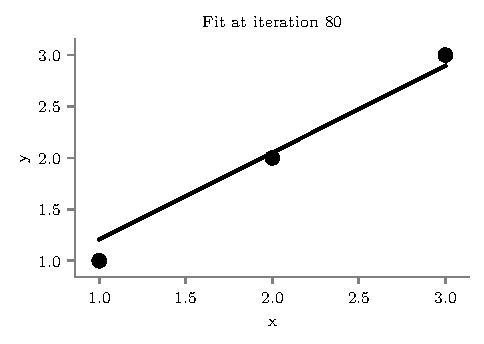
\includegraphics[width=0.7\linewidth]{gradient-descent/fit-iteration-80.pdf}
\end{figure}
\end{frame}

\begin{frame}{Fit at iteration 100}
\begin{figure}
	\centering
	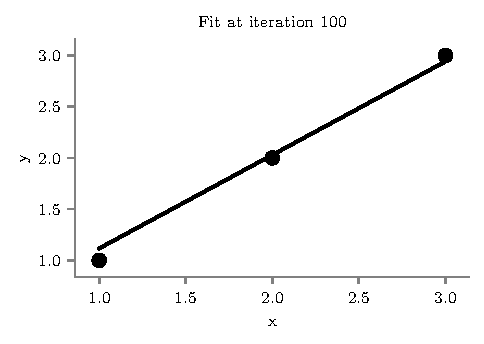
\includegraphics[width=0.7\linewidth]{gradient-descent/fit-iteration-100.pdf}
\end{figure}
\end{frame}

\begin{frame}{Fit at iteration 120}
\begin{figure}
	\centering
	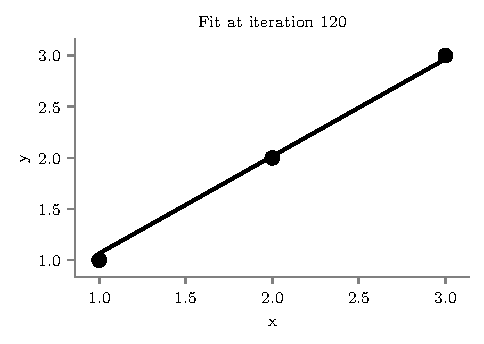
\includegraphics[width=0.7\linewidth]{gradient-descent/fit-iteration-120.pdf}
\end{figure}
\end{frame}

\begin{frame}{Fit at iteration 140}
\begin{figure}
	\centering
	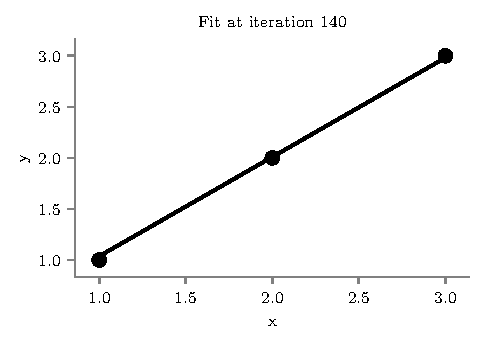
\includegraphics[width=0.7\linewidth]{gradient-descent/fit-iteration-140.pdf}
\end{figure}
\end{frame}

\begin{frame}{Fit at iteration 160}
\begin{figure}
	\centering
	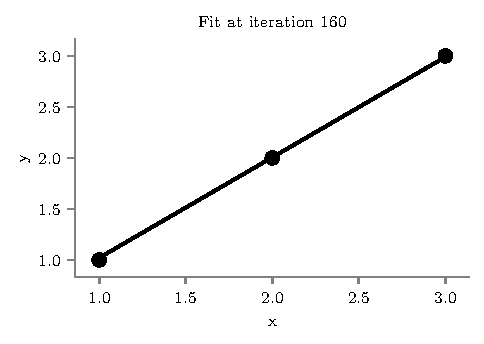
\includegraphics[width=0.7\linewidth]{gradient-descent/fit-iteration-160.pdf}
\end{figure}
\end{frame}

\begin{frame}{Fit at iteration 180}
\begin{figure}
	\centering
	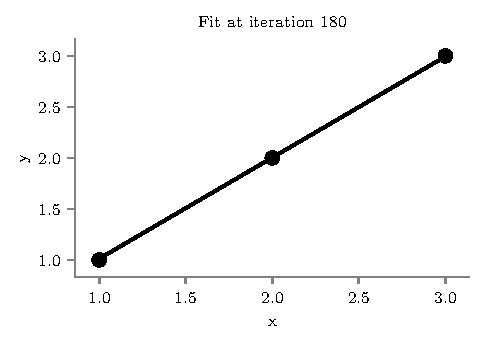
\includegraphics[width=0.7\linewidth]{gradient-descent/fit-iteration-180.pdf}
\end{figure}
\end{frame}

%	\begin{frame}{Gradient Descent for Parabola }
%		Start with a random starting point for x.\\ Say x = 4.1\\
%		$\cfrac{\partial}{\partial x}(x^2) = 2x$
%		
%		\begin{itemize}
%			\item<+-> $x = 4.10 - \alpha * 2 * 4.10 $; $x = 3.68$
%			\item<+-> $x = 3.68 - \alpha * 2 *3.68 $; $x = 3.32$
%			\item<+-> $x = 3.32 - \alpha * 2 *3.32 $; $x = 2.98$
%			\item<+-> \dots
%		\end{itemize}
%		
%		
%	\end{frame}

	

	
	
	

	

	
	\begin{frame}{Gradient Descent vs SGD}

	
	
	
	Vanilla Gradient Descent
	\begin{itemize}[<+->]
		\item 
		in Vanilla (Batch) gradient descent: We update params after going through all the data 
		\item Smooth curve for Iteration vs Cost
		\item For a single update, it needs to compute the gradient over all the samples. Hence takes more time
		
	\end{itemize}
	
	Stochastic Gradient Descent
	\begin{itemize}[<+->]
		\item In SGD, we update parameters after seeing each each point
		\item Noisier curve for iteration vs cost 
		\item  For a single update, it computes the gradient over one example. Hence lesser time
	\end{itemize}
	
	
\end{frame}

	
	
	
	
	\begin{frame}{}
	\begin{columns}
	\begin{column}{0.5\textwidth}{\underline{Gradient Descent}}
		\begin{itemize}
			\item Slower in speed\\ (Needs to see many examples before update)
			\item Smooth convergence
			\item $iterations = epochs$
		\end{itemize}
		\vspace{0.5cm}
		\centering
		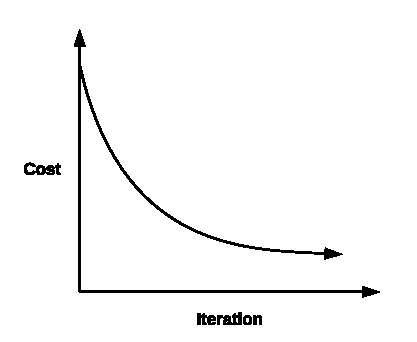
\includegraphics[width = 0.8\textwidth]{sgd-gd/imgs/gd-cost-iter-curve}
	\end{column}
	
	\begin{column}{0.5\textwidth}{\underline{Stochastic Gradient Descent}}
		\begin{itemize}
			\item Faster in speed
			\vspace{0.5cm}
			\item Noisy convergence
			\item $iterations = epochs \times examples$
		\end{itemize}
		\vspace{0.5cm}
		\centering
		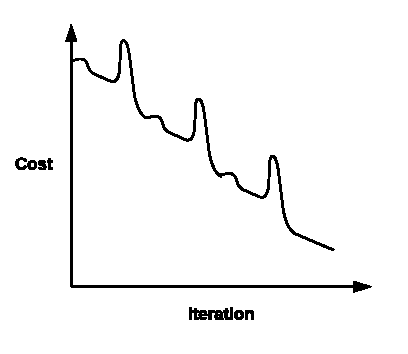
\includegraphics[width = 0.8\textwidth]{sgd-gd/imgs/sgd-cost-iter-curve}
	\end{column}
\end{columns}
\end{frame}

		

\begin{frame}{Stochastic Gradient Descent : Example}
Learn $y = \theta_0 + \theta_1 x$ on following dataset, using SGD where initially $(\theta_0, \theta_1) = (4,0)$ and step-size, $\alpha  = 0.1$, for 1 epoch (3 iterations). 
\begin{table}[]
	\centering
	\label{tab:my-table}
	\begin{tabular}{|c|c|}
		\hline
		\textbf{x} & \textbf{y} \\ \hline
		2 & 2 \\ \hline
		3 & 3 \\ \hline
		1 & 1 \\ \hline
	\end{tabular}
\end{table}
\end{frame}

\begin{frame}{Stochastic Gradient Descent : Example}
Our predictor, $\hat{y} = \theta_0 + \theta_1x$\\
\vspace{1cm}
Error for $i^{th}$ datapoint, $e_i = y_i - \hat{y_i}$\\
$e_1 = 1 - \theta_0 - \theta_1$ \\
$e_2 = 2 - \theta_0 - 2\theta_1$ \\
$e_3 = 3 - \theta_0 - 3\theta_1$ \\

\vspace{1cm}
While using SGD, we compute the MSE using only 1 datapoint per iteration. \\
So MSE is $e_1^2$ for iteration 1 and $e_2^2$ for iteration 2.
\end{frame}


\begin{frame}{Stochastic Gradient Descent : Example}
\textbf{For Iteration $i$}\\
\vspace{1cm}
$\dfrac{\partial MSE}{\partial \theta_0} = 2\left( y_i - \theta_0 -\theta_1x_i \right)\left(-1\right) = 2e_i\left(-1\right)$ \\
\vspace{2cm}
$\dfrac{\partial MSE}{\partial \theta_1} = 2\left( y_i - \theta_0 -\theta_1x_i \right)\left(-x_i\right) = 2e_i\left(-x_i\right)$ 
\end{frame}

\begin{frame}{Stochastic Gradient Descent : Example}
\textbf{Iteration 1}\\
\vspace{0.5cm}
$\theta_0 = \theta_0 - \alpha\dfrac{\partial MSE}{\partial \theta_0}$\\ 
\vspace{0.5cm}
\only<2->{
$\theta_0 = 4 - 0.1 \times 2 \times \left( 2 - (4 + 0) \right)(-1)$\\

\vspace{0.5cm}
$\theta_0 = 3.6$
\vspace{0.5cm}
}

$\theta_1 = \theta_1 - \alpha\dfrac{\partial MSE}{\partial \theta_1}$\\ 
\vspace{0.5cm}
\only<3->{
$\theta_1 = 0 - 0.1 \times 2 \times \left( 2 - (4 + 0) \right)(-2)$\\
\vspace{0.5cm}
$\theta_1 = -0.8$
}
\end{frame}

\begin{frame}{Stochastic Gradient Descent : Example}
\textbf{Iteration 2}\\
\vspace{0.5cm}
$\theta_0 = \theta_0 - \alpha\dfrac{\partial MSE}{\partial \theta_0}$\\ 
\vspace{0.5cm}
\only<2->{
$\theta_0 = 3.6 - 0.1 \times 2 \times \left( 3 - (3.6 - 0.8 \times 3 )\right)(-1) $\\

\vspace{0.5cm}
$\theta_0 = 3.96$
\vspace{0.5cm}
}

$\theta_1 = \theta_1 - \alpha\dfrac{\partial MSE}{\partial \theta_1}$\\ 
\vspace{0.5cm}
\only<3->{
$\theta_0 = -0.8 - 0.1 \times 2 \times \left( 3 - (3.6 - 0.8 \times 3 ) \right)(-3)$\\
\vspace{0.5cm}
$\theta_1 = 0.28$
}
\end{frame}

\begin{frame}{Stochastic Gradient Descent : Example}
\textbf{Iteration 3}\\
\vspace{0.5cm}
$\theta_0 = \theta_0 - \alpha\dfrac{\partial MSE}{\partial \theta_0}$\\ 
\vspace{0.5cm}
\only<2->{
$\theta_0 = 3.96 - 0.1 \times 2 \times \left( 1 - (3.96 + 0.28 \times 1 )\right)(-1) $\\

\vspace{0.5cm}
$\theta_0 = 3.312$
\vspace{0.5cm}
}

$\theta_1 = \theta_1 - \alpha\dfrac{\partial MSE}{\partial \theta_1}$\\ 
\vspace{0.5cm}
\only<3->{
$\theta_0 = 0.28 - 0.1 \times 2 \times \left( 1 - (3.96 + 0.28 \times 1 )\right)(-1) $\\
\vspace{0.5cm}
$\theta_1 = -0.368$
}
\end{frame}

	
	\begin{frame}{Mini-Batch Gradient Descent}
		
		In mini-batch gradient descent, we compute the gradient over a mini-batch of samples, thereby getting the best of both worlds.
		
	\end{frame}
	
	\begin{frame}{When to use Gradient Descent}
		
		
		Gradient Descent
		\begin{itemize}
			\item Good for online setting (more data over time, no need to create new matrices!)
			\item Good for large data
		\end{itemize}
		
		
		Normal systems
		\begin{itemize}
			\item Good for simple data
			\item No need to worry about learning rates, etc
			\item Non trivial to solve
		\end{itemize}
	\end{frame}
	
	
	
	\begin{frame}{Projected Gradient Descent}
		For the $\theta_{i}$
		
		\begin{equation*}
		\theta_{i} = max(\theta_{i} - \alpha \cfrac{\partial \epsilon (\theta_{0},\theta_{1},...)}{ \nabla  \theta_{i}},0)
		\end{equation*}
	\end{frame}
	

	
	\begin{frame}{When to Stop iterating?}
		We stop iterating when the MSE at epoch $i$ is close to the loss at MSE at epoch $i+1$.
	\end{frame}
	
\end{document}